\documentclass[mathNotesPreamble]{subfiles}
\begin{document}
\relscale{1.4} %TODO
\section{15.5: Directional Derivatives and the Gradient}
  Directional derivatives allow us to evaluate the rate of change of a function $f(x,y)$ along any direction (not just parallel with the $x$-axis and $y$-axis).
  \vspace*{\stretch{1}}

  \begin{center}
    \hspace*{\stretch{1}}
    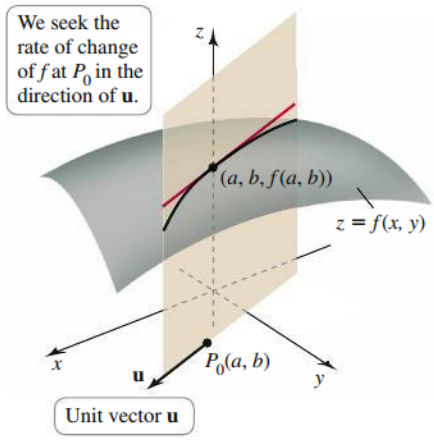
\includegraphics[width=0.375\linewidth]{images/briggs_15_05/fig15_45}
    \hspace*{\stretch{1}}
    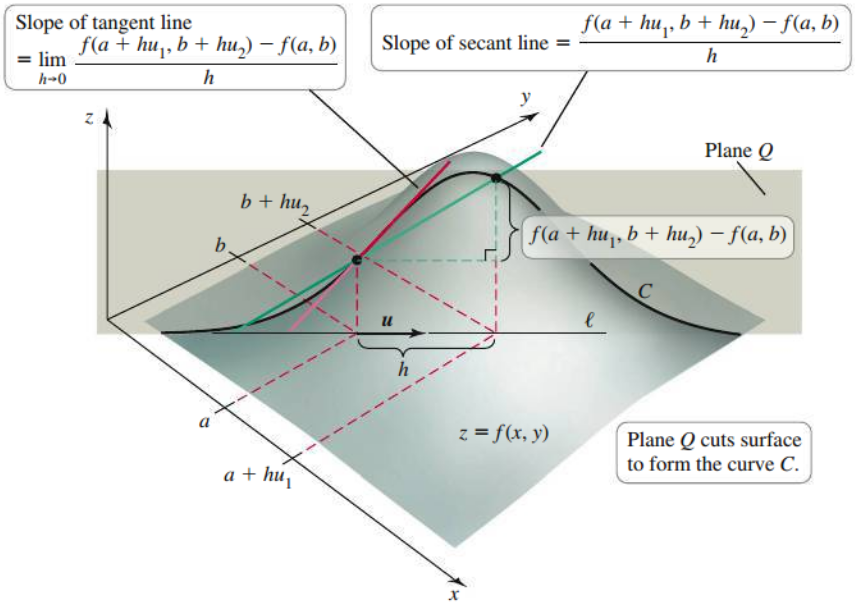
\includegraphics[width=0.5\linewidth]{images/briggs_15_05/fig15_47}
    \hspace*{\stretch{1}}
  \end{center}
  \vspace*{\stretch{1}}

  \begin{defn*}[Directional Derivative]
    Let $f$ be differentiable at $(a,b)$ and let $\vecu=\bracket{u_1,u_2}$ be a unit vector in the $xy$-plane. The \textbf{directional derivative of $f$ at $(a,b)$ in the direction of $u$} is 
      \[D_\vecu f(a,b)=\lim_{h\to 0} \frac{f(a+hu_1,b+hu_2)-f(a,b)}{h},\]
    provided the limit exists.
  \end{defn*}
  \pagebreak

  \noindent
  \fbox{\parbox{0.9875\linewidth}{
    \textbf{Theorem 15.10: Directional Derivative}\\
    Let $f$ be differentiable at $(a,b)$ and let $\vecu=\bracket{u_1,u_2}$ be a unit vector in the $xy$-plane. The \textbf{directional derivative of $f$ at $(a,b)$ in the direction of $\vecu$} is
      \[D_\vecu f(a,b)=\bracket{f_x(a,b), f_y(a,b)}\cdot\bracket{u_1, u_2}.\]
  }}

  \begin{defn*}[Gradient (Two Dimensions)]
    Let $f$ be differentiable at the point $(x,y)$. The \textbf{gradient} of $f$ at $(x,y)$ is the vector-valued function
      \[\grad f(x,y)=\bracket{f_x(x,y),\,f_y(x,y)}=f_x(x,y)\bfi+f_y(x,y)\bfj.\]
  \end{defn*}

  \noindent
  \fbox{\parbox{0.9875\linewidth}{
    \textbf{Theorem 15.11: Directions of Change}\\
    Let $f$ be differentiable at $(a,b)$ with $\grad f(a,b)\neq \bfO$.
    \begin{enumerate}
      \item 
        $f$ has its maximum rate of increase at $(a,b)$ in the direction of the gradient $\grad f(a,b)$. The rate of change in this direction is $\abs{\grad f(a,b)}$.
      \item 
        $f$ has its maximum rate of decrease at $(a,b)$ in the direction of $-\grad f(a,b)$. The rate of change in this direction is $-\abs{\grad f(a,b)}$.
      \item 
        The directional derivative is zero in any direction orthogonal to $\grad f(a,b)$.
    \end{enumerate}
  }}

  \noindent
  \fbox{\parbox{0.9875\linewidth}{
    \textbf{Theorem 15.12: The Gradient and Level Curves}\\
    Given a function $f$ differentiable at $(a,b)$, the line tangent to the level curve of $f$ at $(a,b)$ is orthogonal to the gradient $\grad f(a,b)$, provided $\grad f(a,b)\neq \bfO$.
  }}

  \begin{defn*}[Directional Derivative and Gradient in Three Dimensions]
    Let $f$ be directional at $(a,b,c)$ and let $\vecu=\bracket{u_1,\,u_2,\,u_3}$ be a unit vector. The \textbf{directional derivative of $f$ at $(a,b,c)$ in the direction of $\vecu$} is
      \[D_\vecu (a,b,c)=\lim_{h\to 0} \frac{f(a+hu_1,\,b+hu_2,\,c+hu_3)-f(a,b,c)}{h},\]
    provided this limit exists.\newline
    The \textbf{gradient} of $f$ at this point $(x,y,z)$ is the vector-valued function
      \begin{align*}
        \grad f(x,y,z)&=\bracket{f_x(x,y,z),\,f_y(x,y,z),\,f_z(x,y,z)}\\
          &=f_x(x,y,z)\bfi+f_y(x,y,z)\bfj+f_z(x,y,z)\bfk.
      \end{align*}
  \end{defn*}

  \noindent
  \fbox{\parbox{0.9875\linewidth}{
    \textbf{Theorem 15.13: Directional Derivative and Interpreting the Gradient}\\
    Let $f$ be differentiable at $(a,b,c)$ and let $\vecu=\bracket{u_1,\,u_2,\,u_3}$ be a unit vector. The directional derivative of $f$ at $(a,b,c)$ in the direction of $\vecu$ is
    \begin{align*}
      D_\vecu f(a,b,c)&=\grad f(a,b,c)\cdot \vecu\\
        &=\bracket{f_x(a,b,c),\, f_y(a,b,c),\,f_z(a,b,c)}\cdot\bracket{u_1,\,u_2,\,u_3}.
    \end{align*}
    Assuming $\grad f(a,b,c)\neq \bfO$, the gradient in three dimensions has the following properties.
    \begin{enumerate}
      \item 
        $f$ has its maximum rate of increase at $(a,b,c)$ in the direction of the gradient $\grad f(a,b,c)$ and the rate of change in this direction is $\abs{\grad f(a,b,c)}$.
      \item 
        $f$ has its maximum rate of decrease at $(a,b,c)$ in the direction of $-\grad f(a,b,c)$ and the rate of change in this direction is $-\abs{\grad f(a,b,c)}$.
      \item 
        The directional derivative is zero in any direction orthogonal to $\grad f(a,b,c)$.
    \end{enumerate}
  }}

  \pagebreak
  
\end{document}